	\section{Il Data Werahouse}
Un \textbf{Data Warehouse} è una collezione di dati al supporto del processo decisionale con le seguenti caratteristiche:
\begin{itemize}
	\item
	È orientata ai soggetti di interesse (\textbf{subject oriented}): nasce per contrapposizione al mondo operazionale, in cui siamo application oriented. Infatti, quando si progettano database operazionali questi sono progettati finalizzati ad un’applicazione, quindi ad una macro-funzionalità. 
	\begin{figure}[H]
		\centering
		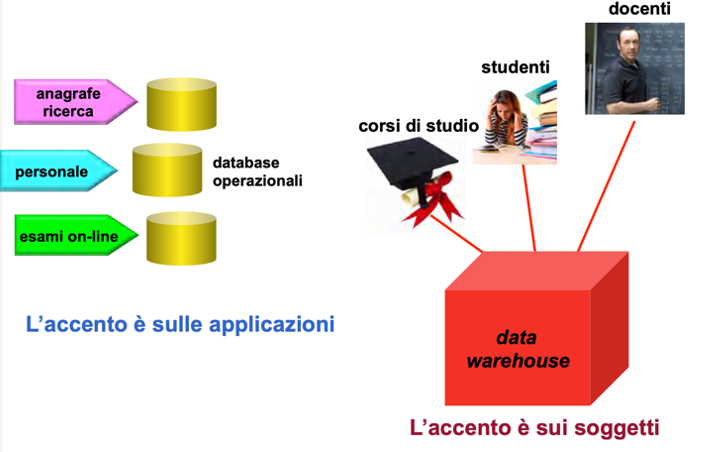
\includegraphics[width=0.7\linewidth]{img/SubjO}
		\caption{Subject Oriented}
		\label{fig:subjor}
	\end{figure}
	
	La conseguenza è che all’interno di ciascuno di questi database, di queste macro-funzionalità, i dati sono consistenti-integrati ma non lo sono rispetto ad altre funzionalità. Il senso di application oriented è che ogni applicazione è potenzialmente un mondo a sé. Quando si passa al contesto del DW, l’accento è sui soggetti, ovvero i protagonisti del business. A prescindere dalle funzionalità di ciascuno di questi soggetti io riesco a costruire dentro al DW una visiona completa in cui metto insieme tutto quello che quel soggetto fa o subisce. 
	\item 
	\textbf{È integrata e consistente}: è fondamentale che dentro al DW i dati che provengono dai diversi eterogenei database operazionali vengono combinati e riconciliati tra loro. Per prima cosa devo estrarre i dati, poi validare e pulire (eliminare per quando possibile gli errori), quindi li devo trasformare perché li devo integrare tra loro oltre che metterli in forma multidimensionale. Solo dopo posso caricarli nel data werahouse.
	Nei DB operazionali si può pensare che sia rappresentato in ogni istante una fotografia del business, i dati infatti sono soggetti ad aggiornamenti. Nel data werahouse buona parte delle query OLAP lavorano sui trend temporali. Ho bisogno di mantenere la storia, e immagino che l’ETL scatti una fotografia del business (DB operazionale) e la carica nel DW mettendola in coda a quelle precedenti. 
	\item 
	\textbf{È rappresentativa del tempo}
	\item 
	\textbf{Non volatile}: nel caso del DB operazionale il carico di lavoro OLTP è in lettura e in scrittura. Quindi in SQL, oltre alle SELECT, abbiamo INSERT, UPDATE e DELETE. Dentro al data werahouse, il carico di lavoro è in solo lettura. Ci sarà un momento in cui però andrò a scrivere, quando avvio l’ETL. In questo modo non ho problemi di accesso concorrenti in scrittura, e quindi non si pone il problema della transazione. L’unico problema che si ha è il query-throughput, cioè riuscire a dare buone prestazioni a diversi utenti che lanciano contemporaneamente delle query OLAP.
\end{itemize}
\begin{figure}
	\centering
	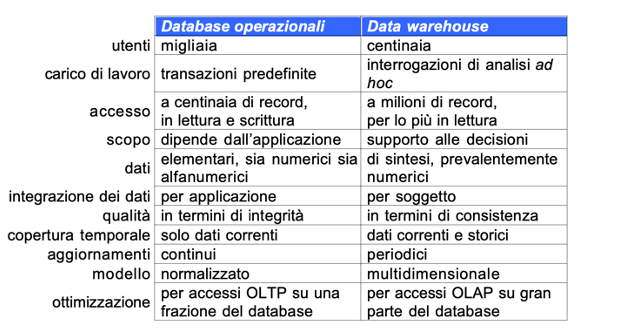
\includegraphics[width=0.9\linewidth]{img/DBeDW}
	\caption{Differenza DB operazionali e DW}
	\label{fig:differenze}
\end{figure}
\subsection{Architetture di Data Werahouse}
\subsubsection{I requisiti}
\begin{itemize}
	\item 
	\textbf{Separazione}: elaborazione analitica e quella transazionale devono essere mantenute il più possibile separate. 
	\item
	\textbf{Scalabilità}: con una crescita delle necessità, maggior volume dati e numero di utenti, si riesca a ridimensionare l’architettura HW-SW senza particolari problemi, non creando colli di bottiglia. 
	\item
	\textbf{Estendibilità}: poter aggiungere facilmente nuove applicazioni che interoperano con le precedenti
	\item
	\textbf{Sicurezza}: i dati che finiscono nel DW sono di importanza strategica per l’azienda; gli utenti del DW non possono vedere tutto ma accedono solo a porzioni più o meno ampie del DW
	\item
	\textbf{Amministrabilità}: la complessità dell’attività amministrativa non deve risultare troppo complesso da gestire
\end{itemize}
\subsubsection{Classificazione}

Una prima classificazione delle architetture è di tipo strutturale, in cui distinguiamo tre tipi di architetture in base al numero di livelli fisici presenti nell’architettura. 
La prima architettura, quella ad un livello, in figura \ref{fig:arch1} presenta un solo livello fisico, quello delle sorgenti in cui tengo traccia dei dati operazionali. Non si ha un DW fisico e in mezzo presenta un \textbf{middleware} (un sistema) che prende le query OLAP, le scrive sul DB operazionale, le esegue e restituisce i dati all’utente. Non rispetta il requisito della separazione.
\begin{figure}[H]
	\centering
	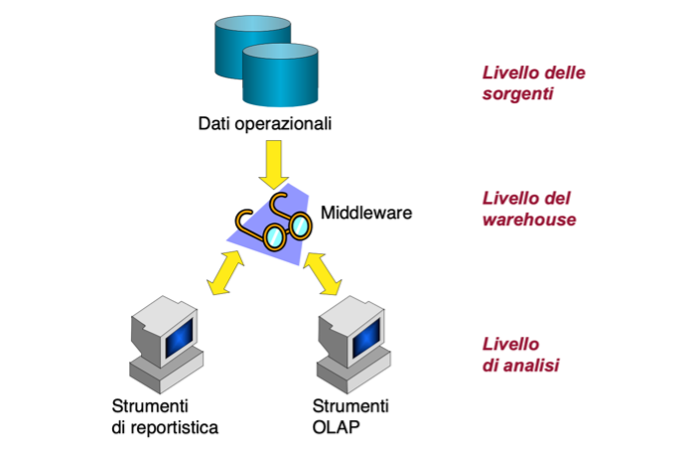
\includegraphics[width=0.6\linewidth]{img/arch1}
	\caption{Architettura ad un livello}
	\label{fig:arch1}
\end{figure}

L’architettura a due livelli presenta due livelli fisici, il livello della sorgente e il livello del werahouse e pertanto il requisito della separazione è soddisfatto. In mezzo c’è l’ETL che ha il compito di filtrare, estrare il distillato dei dati e caricarlo dentro al data werahouse. Dal livello di Dara Werahouse si accede al livello di analisi attraverso strumenti di reportistica, strumenti OLAP, analisi what-if ecc. I cilindri arancioni sono i data mart, ovvero porzioni di DW. Ciascun data mart è relativo ad una specifica area aziendale e quindi viene utilizzato da un sottoinsieme degli utenti. L’utilizzo dei data mart facilita il controllo degli accessi, perché il DW è già partizionato in data mart legati ad aree aziendali. Il data mart è l'incremento di progettazione e costruzione dei DW. Quindi questi vengono progettati e costruiti un data mart alla volta. 
\begin{figure}[H]
	\centering
	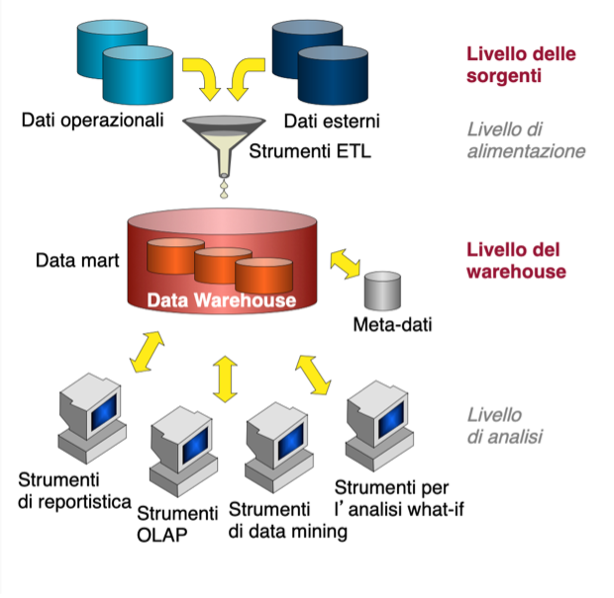
\includegraphics[width=0.6\linewidth]{img/arch2}
	\caption{Architettura a due livelli}
	\label{fig:arch2}
\end{figure}

L’architettura a tre livelli, in cui il nuovo livello fisico è quello dell’alimentazione, ovvero quello dell’ETL, la quale non viene vista solo come una procedura, ma ha il compito di “appoggiare” i risultati su un ulteriore DB, detto \textbf{ODS (Operation Data Store}). È un DB con dati operazionali, elementari, volatili, che si trovano a valle dell’ETL; quindi, sono dati puliti in quando gli errori sono stati già corretti. Successivamente vi è la fase di caricamento, i dati vengono estratti dall’ODS, messi in forma multidimensionale, aggregati per fare sintesi, e scritti dentro al DW. L'ODS assume un'importanza perchè questo è il luogo perfetto per lanciare la reportistica operativa. Infatti, nella piramide della BI, si nota che tra il livello inferiore dei dati e quello del data werahouse c’è proprio l’ODS. Cosa si intende per reportisca operativa? Un report è in generale, un risultato che si ottiene da una manipolazione dei dati. Il report strategico per i manager è di più alto livello; quindi, lavora con dati raggruppati (trend temporali ecc). Il report operativo è sempre una query in lettura, ma richiede un livello di dettaglio con solo dati correnti. Dunque, non serve ai livelli strategici ma ai livelli tattici. Spesso tali report non sono stati previsti nel momento in cui è stato progettato il DB relazionale, quindi non sono implementati. L’ODS è normalizzato, mentre il data werahouse no. \\

La seconda classificazione delle architetture  le distingue a seconda del modo con cui realizzano o non realizzano un’integrazione del dato a livello aziendale. Tali architetture sono:
\begin{itemize}
	\item 
	\textbf{Data mart indipendenti}: l’idea è che per ogni area aziendale ho fatto un progetto verticale senza tenere conto delle altre aree aziendali. Ho diversi data mart progettati indipendentemente gli uni dagli altri. In questo tipo di architettura i data mart vengono anche chiamati silos (compartimenti che non si parlano tra loro). Ad esempio voglio valutare un docente che tenga conto di quanti esami fa in un anno, di quanti articoli scrive, del suo ruolo, dello stipendio. Tutti questi numeri vengono da dati mart diversi, quindi per poter calcolare questo numero su ciascun docente ho bisogno di incrociare questi dati (JOIN). Il problema è che i data mart sono stati progettati separatamente e dunque il collegamento non è fattibile, perché ciascun data mart descrive il docente in maniera differente. L’architettura data mart indipendenti è veloce, relativamente economica, ma non è una buona architettura in quando non soddisfa il requisito di integrazione enterprise. 
	\begin{figure}[H]
		\centering
		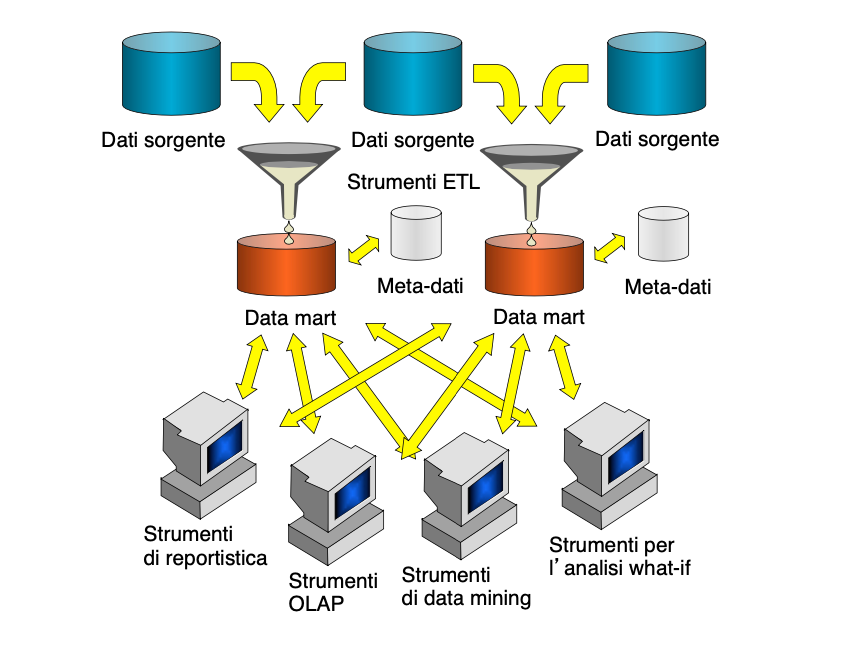
\includegraphics[width=0.5\linewidth]{img/DMind}
		\caption{Data Mart Indipendenti}
		\label{fig:dmind}
	\end{figure}
	\item 
	\textbf{Data mart bus}: simile all’architettura precedente con la differenza del blocco delle \textbf{dimensioni conforme}. Il trucco sta nel fatto che pur avendo dei mondi verticali si preveda all’inizio del progetto, un binario comune, che renda possibile l’integrazione dei data mart a posteriori. Quindi la enterprise view integrata del business la realizzo a livello logico. Le dimensioni conforme sono i concetti primari di business condivisi dalla maggior parte dei data mart. Prima di iniziare a realizzare il data mart prendo un cliente chiave da ciascuna area aziendale finché non si accordano su una definizione univoca sui diversi concetti chiave del business (dimensioni conforme). Dopo di che ogni reparto è libero di costruirsi il data mart come vuole ma con il vincolo di rispettare le dimensioni conformi. Il bello di questa architettura è che in ogni data mart posso decidere se usare un’architettura a due o tre livelli.
	\begin{figure}[H]
		\centering
		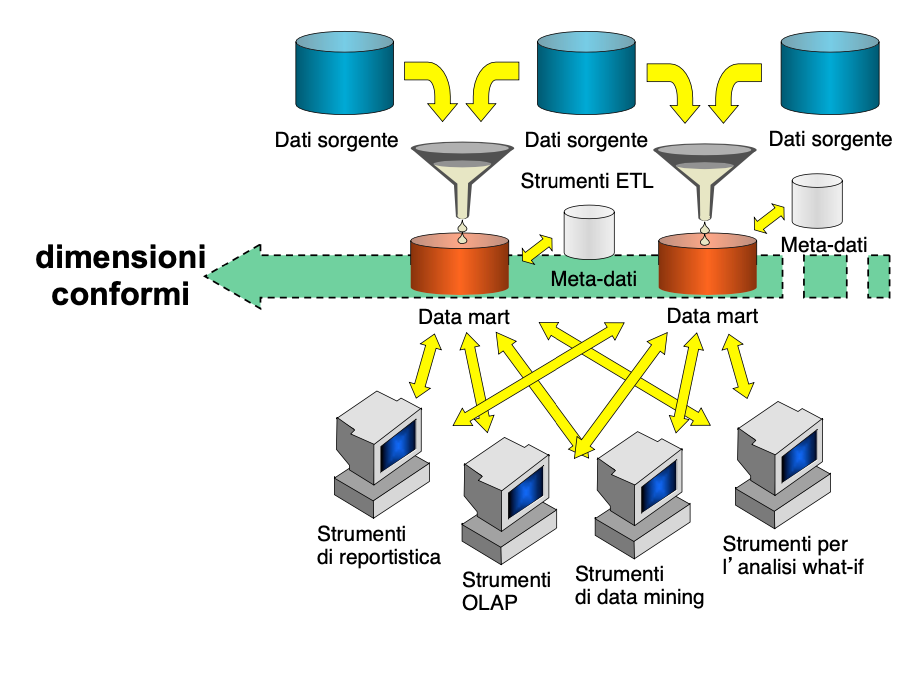
\includegraphics[width=0.5\linewidth]{img/DMcon}
		\caption{Data Mart Bus}
		\label{fig:dmbus}
	\end{figure}
	\item 
	\textbf{Hub-and-spoke}: questo tipo di architettura realizza nativamente un enterpise view. Per farlo utilizza un ODS enterprise \footnote{Un ODS a livello enterprise è relativamente complesso da progettare, perché bisogna mettere insieme idee e requisiti di tutti gli utenti aziendali e non solo ai principali soggetti del business} che copre tutta l’azienda, integrando tutti i dati aziendali, estraendo, solo dopo le singole informazioni per i vari data mart che sono allora volta integrabili. L’hub and spoke rispetto al data mart bus risulta essere più costoso.
	\begin{figure}[H]
		\centering
		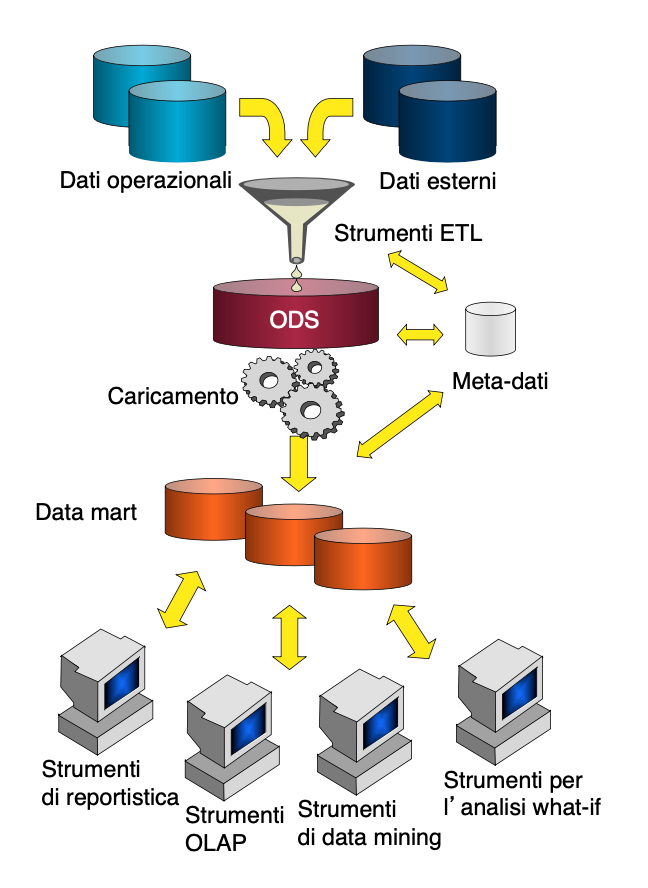
\includegraphics[width=0.2\linewidth]{img/hubandspoke}
		\caption{Hub and spoke}
		\label{fig:hubandspoke}
	\end{figure}
	\item 
	\textbf{Federazione}: il Data Werahouse federato si utilizza in due contesti: il primo è quello dinamico (fusioni-acquisizioni). L’esempio più eclatante è quello delle banche che uniscono rispettivamente i due business. Potrei mantenere entrambi i data werahouse ma prima o poi bisogna dare una versione unificata. Per fare ciò viene creato un DW di secondo livello. Grazie a ciò riesco ad incorporare nuovi DW senza doverli rifare da capo. L’architettura federata serve però anche come patch ad un’architettura data mart indipendente, progettando un DW di secondo livello, dove introducendo un livello di ETL ulteriore riesco a mettere insieme le cose. 
	\begin{figure}[H]
		\centering
		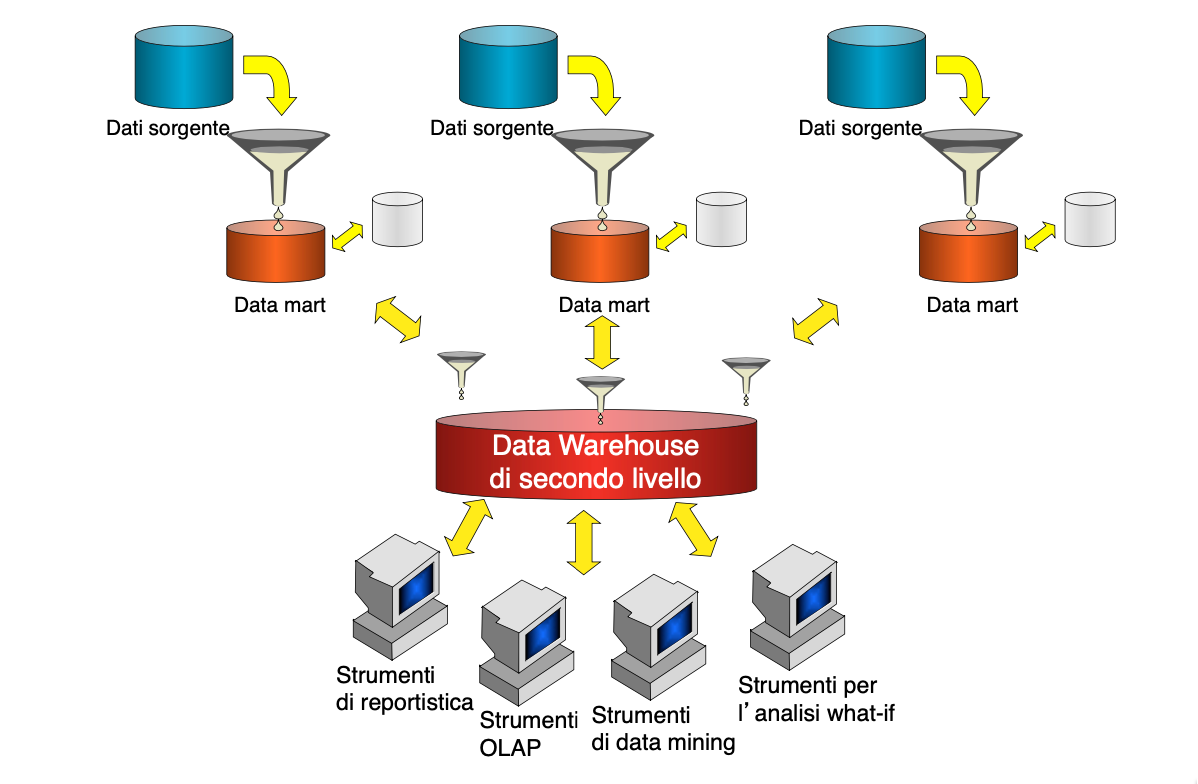
\includegraphics[width=0.7\linewidth]{img/fede}
		\caption{Federazione}
		\label{fig:federazione}
		
	\end{figure}
\end{itemize}
\subsubsection{Fattori di scelta dell'architettura}
La scelta dell’architettura dipende da diversi aspetti:
\begin{enumerate}
	\item 
	Bisogna capire quanto alta o bassa è la sponsorship del progetto, chi è che vuole il data werahouse? Il CEO o il mio capo reparto? Nel primo caso devo adottare un’architettura enterprise, nel secondo caso potrei optare per una data mart indipendente ma essere pronto al fatto che dovrò rimediare
	\item 
	Quanto le diverse unità organizzative in azienda sono legate tra di loro o meno (hub-and-spoke) o (data mart indipendent o bus)
	\item 
	Urgenza del progetto di data werahousing
	\item 
	Compatibilità con piattaforme esistenti: nei casi reali la software selection non si fa a 360 gradi, perché nella mia azienda ho già oracle o ibm e poiché sono orientato già verso uno stack tecnologico ho particolari vantaggi nel continuare a sposare quell’azienda.
\end{enumerate}